\documentclass[CO_LUU_CHAT_NANG_CAO.tex]{subfiles}

\begin{document}
\chapter{PHƯƠNG TRÌNH NAVIER-STOKES}
\section{Sự nhớt, tenxơ ứng suất và phương trình Navier-Stokes}
Độ nhớt là một thước đo mức độ phân tán động lượng bởi vì cấu trúc vi mô của lưu chất thực, do đó hiệu ứng của nó là tạo ra sự cản trở chuyển động trượt. Chúng ta hãy cùng tìm hiểu thông qua ví dụ sau.
\begin{exmp}
    Một hình trụ có trục hướng thẳng đứng và bán kính $R$ chứa đầy một chất lỏng thực. Hệ ban đầu ở trạng thái nghỉ và chúng ta xoay hình trụ với vận tốc góc cố định $\Omega$. Trước hết, chỉ các lớp chất lỏng liền kề với thành hình trụ chuyển động với vận tốc góc của hình trụ. Dòng chảy truyền theo từng lớp từ ngoài vào trong, theo thời gian, chất lỏng quay với vận tốc góc đều và bằng vận tốc của hình trụ. Điều này được thấy rõ trong Hình \ref{ROTATION_CYLINDER}
    \begin{figure}[h!]
        \centering
        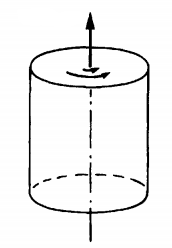
\includegraphics[scale=1]{ROTATION_CYLINDER.png}
        \caption{Hình trụ quay và vận tốc của các lớp lưu chất.}
        \label{ROTATION_CYLINDER}
    \end{figure}
\end{exmp}

Chúng ta đã biết rằng tenxơ ứng suất, $\deuxtenseur{\sigma}$ của một phần tử thể tích $\Omega$ định tâm tại điểm $(x,y,z)$ của một môi trường liên tục là một tenxơ hạng hai hiệp biến ba chiều. Navier và Stokes đã phân tích tenxơ thành tổng của một thành phần cầu và thành phần lệch :
\begin{equation}
    \begin{aligned}
        \deuxtenseur{\sigma} = \deuxtenseur{s} - \deuxtenseur{d} 
    \end{aligned}
\end{equation}
trong đó, tenseur cầu $\displaystyle\deuxtenseur d = -p\deuxtenseur{\mathbbm{1}} = \frac{\text{tr}\deuxtenseur\sigma}{3}\deuxtenseur{\mathbbm{1}}$.

Một cách tổng quát, chúng ta có thể liên hệ tenxơ ứng suất lệch với tenxơ tốc độ biến dạng dưới dạng :
\begin{equation}
    \begin{aligned}
        {s}_{ij} = M_{ijkl}{\dot{\varepsilon}}_{kl}
    \end{aligned}
\end{equation}

Đối với một lưu chất đẳng hướng, chúng ta đặt ra các giả thiết sau :
\begin{itemize}
    \item Tenxơ ứng suất là một hàm tuyến tính của tenxơ tốc độ biến dạng.
    \item Ở trạng thái nghỉ, gradient của tenxơ lệch phải triệt tiêu (giống với trường hợp có áp suất thủy tĩnh).
\end{itemize}
Lúc này, chúng ta có :
\begin{equation}
    \begin{aligned}
        M_{ijkl}=a\delta_{ik}\delta_{jl}+b\delta_{il}\delta_{jk}+a\delta_{ij}\delta_{kl}
    \end{aligned}
\end{equation}

Rõ ràng là đối với lưu chất này, nếu dòng chảy là xoay đều với vận tốc góc $\Omega$, vận tốc là bằng với $\vect{\Omega} \wedge \underline{r}$ và tenxơ lệch bị triệt tiêu. Số hạng 
\[2{\dot{\varepsilon}}_{ij}=\frac{{\partial {v_i}}}{{\partial {x_k}}} + \frac{{\partial {v_k}}}{{\partial {x_i}}}\]
là tổ hợp tuyến tính của các số hạng $\displaystyle\frac{{\partial {v_i}}}{{\partial {x_k}}}$ và triệt tiêu khi $\vect{\Omega} \wedge \underline{r}$. Do đó tenxơ lệch phải chứa chỉ các tổ hợp tuyến tính của các đạo hàm $\partial {v_i}/\partial {x_k}$. Hơn nữa, tenxơ lệch là một tenxơ đối xứng, do đó $a=b$ và ${s_{ij}} = a\left( {{{\dot \varepsilon }_{ij}} + {{\dot \varepsilon }_{ji}}} \right) + c{\dot \varepsilon _{ll}}{\delta _{ij}}$. Nếu giới thiệu các hệ số Lamé như trong lý thuyết đàn hồi, chúng ta có thể viết :
\begin{equation}
    \begin{aligned}
        s_{ij}=\mu({\dot{\varepsilon}}_{ij}+{\dot{\varepsilon}}_{ji}-\frac{{\dot{\varepsilon}}_{ll}}{3}\delta_{ij})+(\lambda+\frac{\mu}{3})\dot{\varepsilon}_{ll}\delta_{ij}.
    \end{aligned}
\end{equation}

Nếu viết đưới dạng tenxơ :
\begin{equation}
    \begin{aligned}
        \underline{\underline s}  = 2\mu \left( {\underline{\underline {\dot \varepsilon }}  - \frac{{\underline \nabla   \cdot \underline u }}{3}\underline{\underline {\mathbbm{1}}} } \right) + \left( {\lambda  + \frac{\mu }{3}} \right)\underline \nabla   \cdot \underline u \text{ }\underline{\underline {\mathbbm{1}}}  = 2\mu \left( {\underline{\underline {\dot \varepsilon }}  - \frac{{\underline \nabla   \cdot \underline u }}{3}\underline{\underline {\mathbbm{1}}} } \right) + {\mu _v}\underline \nabla   \cdot \underline u \text{ } \underline{\underline{\mathbbm{1}}}
    \end{aligned}
\end{equation}
hằng số $\mu_v$ được gọi là hằng số nhớt của lưu chất.

Thay thế trực tiếp tenxơ ứng suất vào phương trình động lượng Euler, chúng ta có :
\begin{equation}\label{NAVIER_STOKES_E}
    \begin{aligned}
        \rho \frac{D\underline{u}}{{Dt}} =  - \underline{\nabla} p + \rho\underline{g} + \mu \Delta \underline u  + \frac{1}{3}\mu \underline \nabla  \left( {\underline \nabla   \cdot \underline u } \right)
    \end{aligned}
\end{equation}

Dòng chảy của chất lỏng ở cấp độ vi mô bị chi phối bởi các hiện tượng trong lĩnh vực cơ học thống kê của chất lỏng. Các va chạm được mô tả bằng toán tử va chạm. Nói chung, toán tử va chạm biểu diển va chạm đồng thời giữa nhiều hạt, như vậy thì quá phức tạp. Chỉ trong trường hợp khí loãng mới có thể giới hạn các nghiên cứu về trường hợp va chạm giữa hai hạt. Trong tình huống lý tưởng hóa này, toán tử va chạm có thể được tính gần đúng theo gradient áp suất và laplacian vận tốc, nhân với một hằng số được gọi là độ nhớt. Với phép gần đúng này, chúng ta suy ra phương trình bảo toàn động lượng (phương trình Navier-Stokes).

Quá trình dẫn xuất như vậy đã được thực hiện đối với các khí loãng, do đó việc áp dụng phương trình này cho lưu chất nói chung là một việc hơi kiên cưỡng. Nguyên nhân là do chất lỏng đặc hơn nhiều so với chất khí và do đó được đặc trưng bởi va chạm giữa các cụm hạt. Tuy nhiên, vì không còn sự lựa chọn nào tốt hơn, chúng tôi vẫn sử dụng phương trình Navier-Stokes với độ nhớt không đổi như một mô hình hợp lý cho các dòng lưu chất.

Nguồn gốc của độ nhớt đặt ra giới hạn đối với phạm vi hiệu lực của phương trình Navier-Stokes. Do đó, các hiện tượng trên thang độ dài cở của quảng đường tự do trung bình của không khí ở áp suất khí quyển (cở $10^{-3}$ cm) không thể được mô tả bởi một mô hình liên tục như NSE. Lưu ý tương tự cũng được sử dụng cho sự nhiễu biên độ của dòng chảy rối : một khi chúng ta ở trong một chế độ trong đó sự nhiễu có thể so sánh được với những dao động nhiệt (nhiệt độ hữu hạn) gây ra, mô hình dựa trên phương trình Navier-Stokes không còn phù hợp.

\section{Phương trình Navier-Stokes vô thứ nguyên}
Đôi khi, sẽ thuận thuận tiện hơn khi xem xét dạng vô thứ nguyên của phương trình Navier-Stokes. Vì mục đích đó, chúng tôi giới thiệu độ dài tham chiếu $L$ và vận tốc tham chiếu $U$ cho dòng chảy, và chúng tôi giới thiệu các phép biến đổi sau :
\begin{center}
    \begin{tabular}{|l|c|}
        \hline
        \textbf{Thang đo} & \textbf{Phép biến đổi}\\
        \hline
        Độ dài $L$ : $\displaystyle\underline{x}' = \underline{x}/L$ &$\displaystyle\nabla ' = L\nabla$\\
        \hline
        Tốc độ chảy $U$ & $\displaystyle\underline{u}' = \underline{u}/{U}$ \\
        \hline
        Thời gian $\displaystyle t'={Ut}/{L}={t}/{T'}$ & $\displaystyle{\partial }/{{\partial t}} = {{{1/T'}}}{\partial }/{{\partial t'}}$ \\
        \hline
        Áp suất (khi hiệu ứng động học chi phối) & $\displaystyle{p'} = {p}/{{\rho {U^2}}}$ \\
        \hline
        Áp suất (khi hiệu ứng nhớt chi phối) & $\displaystyle{p'} = {pL}/{{\mu {U}}}$ \\
        \hline
    \end{tabular}
\end{center}

Thay thế các thang đo này vào phương trình (\ref{NAVIER_STOKES_E}), chúng ta thu được phương trình Navier-Stokes vô thứ nguyên trong trường hợp khi hiệu ứng động học chi phối :
\begin{equation}\label{NAVIER_STOKES_ER}
    \begin{aligned}
        \frac{{D'\underline u '}}{{Dt'}} =  - \underline{\nabla}'p' + \frac{1}{{Fr}}{\underline e _z} + \frac{1}{{{\mathop{\rm Re}\nolimits} }}\Delta '\underline u ' + \frac{1}{{3{\mathop{\rm Re}\nolimits} }}\underline{\nabla} '\left( {\underline{\nabla}'\cdot\underline u '} \right)
    \end{aligned}
\end{equation}
trong đó $\displaystyle\frac{{D'}}{{Dt'}} = \frac{{\partial '}}{{\partial t'}} + \underline u ' \cdot \nabla '$ và chúng ta cũng giới thiệu hai số vô thứ nguyên mà chúng ta gọi là \emph{số Reynold} và \emph{số Froud}, chúng được định nghĩa lần lượt như sau :
\begin{equation}\label{REYNOLD_DEF}
    \begin{aligned}
        {\mathop{\rm Re}\nolimits}  = \frac{{\rho UL}}{\mu }
    \end{aligned}
\end{equation}
\begin{equation}\label{FROUD_DEF}
    \begin{aligned}
        Fr = \frac{U}{{\sqrt {gL} }}
    \end{aligned}
\end{equation}
chúng ta sẽ phân tích về vai trò của hai số này trong các phần tiếp theo.

Thông thường, nếu miền bị chiếm bởi lưu chất, $\Omega$, là bị chặn thì có thể chọn $L$ chính là đường kính của miền $\Omega$ hoặc là một độ dài nào đó có độ lớn với cở của độ lớn của kích thước của miền $\Omega$.

Điều này dẫn đến một câu hỏi tự nhiên đó là, với hai dòng chảy khác nhau nhưng có cùng một phương trình Navier-Stokes vô thứ nguyên, liệu chúng ta có thể xem hai dòng chảy này là có cùng một tính chất topo hay không ? Điều này sẽ được giải quyết trong phần \emph{đồng dạng động lực học} và \emph{định lý Buckingham}.

\section{Dòng chảy rối : một lĩnh vực liên ngành}
Trong dòng chảy rối, các đại lượng vật lý trong lưu chất thay đổi một cách nhanh chóng đến nổi việc đo chúng là một việc không thực tế. Do đó, người ta thực hiện một công việc đơn giản hơn đó là đo giá trị trung bình của các đại lượng này, các giá trị có thể được định nghĩa một cách rõ ràng và có thể được tìm lại được bằng thực nghiệm. Điều này dẫn chúng ta đến \emph{quan điểm thống kê} trong việc xem xét phương trình Navier-Stokes.

Phương trình Navier-Stokes là một phương trình vi phân phi tuyến do số hạng đối lưu trong phương trình. Do đó việc giải được nghiệm của phương trình này là bất khả thi ở thời điểm hiện tại. Điều này dẫn đến những cố gắng trong việc xấp xỉ hóa phương trình. 


\end{document}